\chapter{Laboratorio 4}
\noindent In questo laboratorio, si è studiato e simulato il comportamento di un modulatore Mach-Zehnder interferometer (MZI) in silicio.
\section{Determinazione di $\boldsymbol{\Delta n_{eff}(V)}$ e della perdita ottica in funzione della tensione di polarizzazione inversa}
Mediante i grafici relativi alla misurazione della variazione di fase $\Delta\phi(V)$ e della perdita della trasmissione $TL_{dB}(V)$ in funzione della tensione V, 
si sono ottenute delle funzioni che approssimano l'andamento di questi parametri, attraverso lo strumento \texttt{curve fitter} di MATLAB.
\noindent La variazione di fase $\Delta\phi(V)$ è stata approssimata con una funzione a radice quadrata, quindi ha una forma del tipo:
\[
    \Delta\phi(V) = A \sqrt{V} + B
\]
\noindent mentre la perdita della trasmissione $TL_{dB}(V)$ è stata approssimata con una funzione lineare:
\[
    TL_{dB}(V) = A \cdot V + B
\]

\noindent I grafici delle due funzioni fittanti sono riportati nella Figura \ref{fig:fit_dphi_TL}.

\begin{figure}[!h]
    \centering
    \begin{subfigure}[b]{0.49\textwidth}
        \centering
        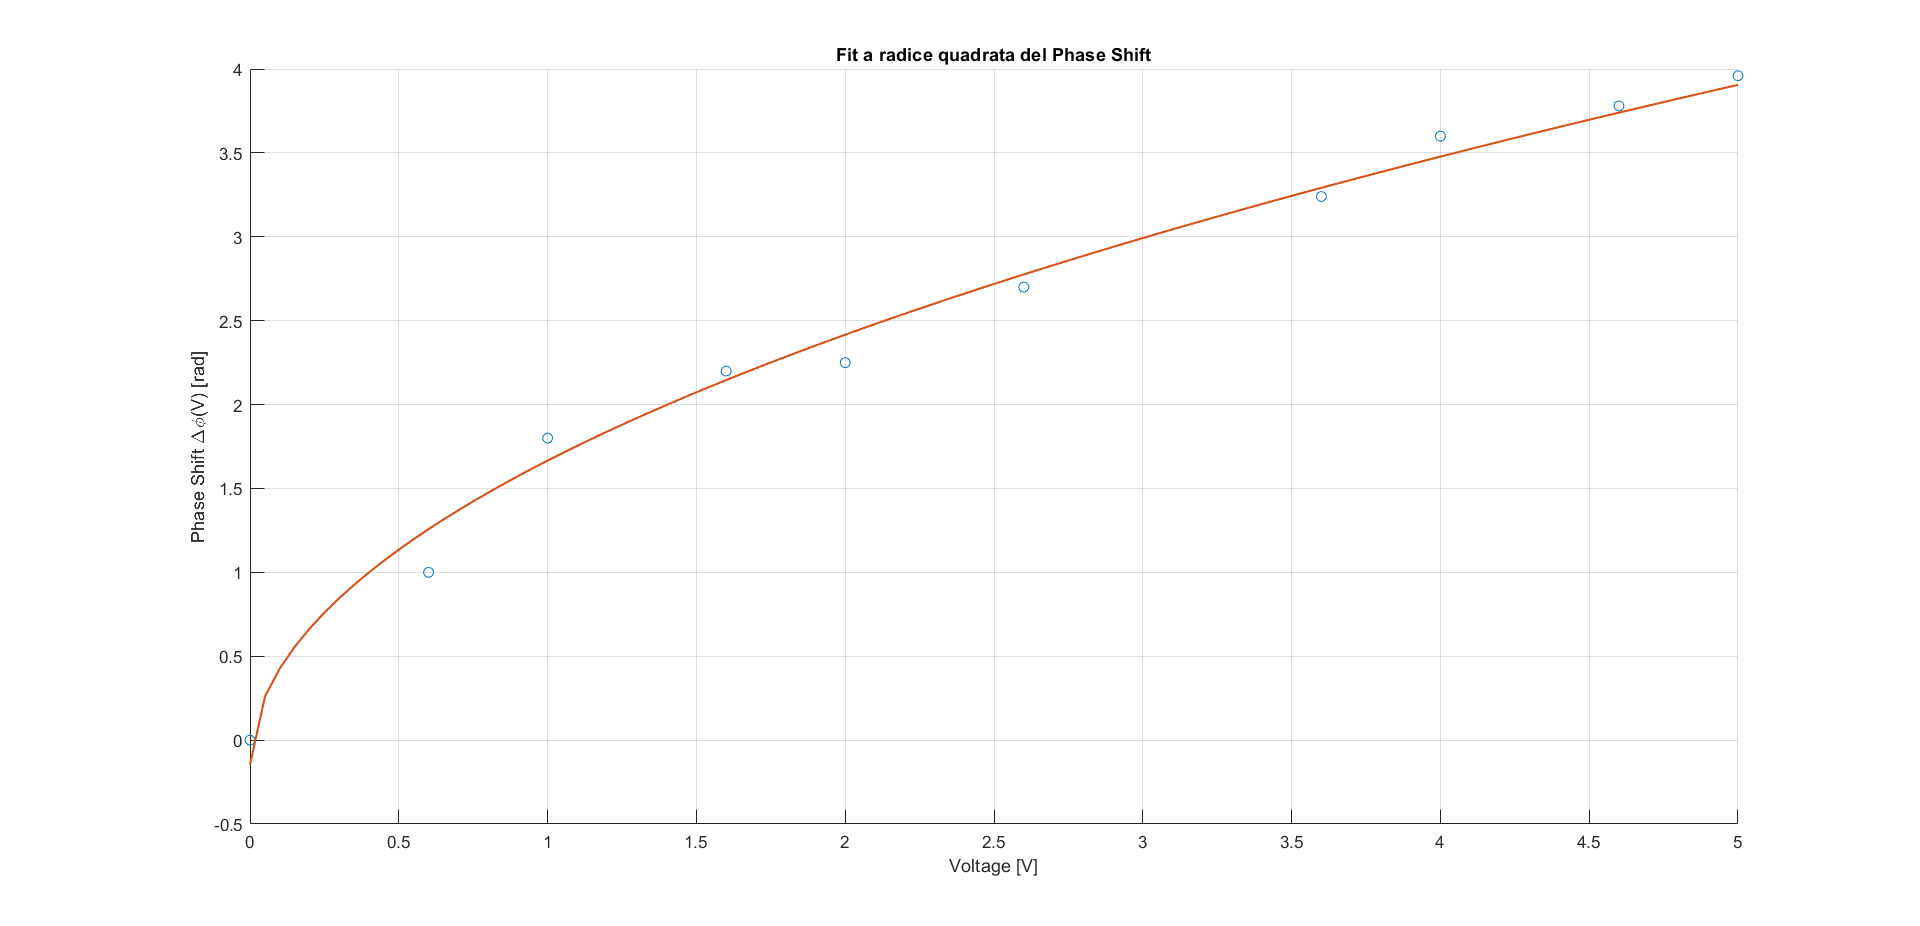
\includegraphics[width=\textwidth]{lab4/Images/fit_PS.png}
        \caption{Fit a radice quadrata di $\Delta\phi(V)$}
        \label{fig:fit_PS}
    \end{subfigure}
    \hfill
    \begin{subfigure}[b]{0.49\textwidth}
        \centering
        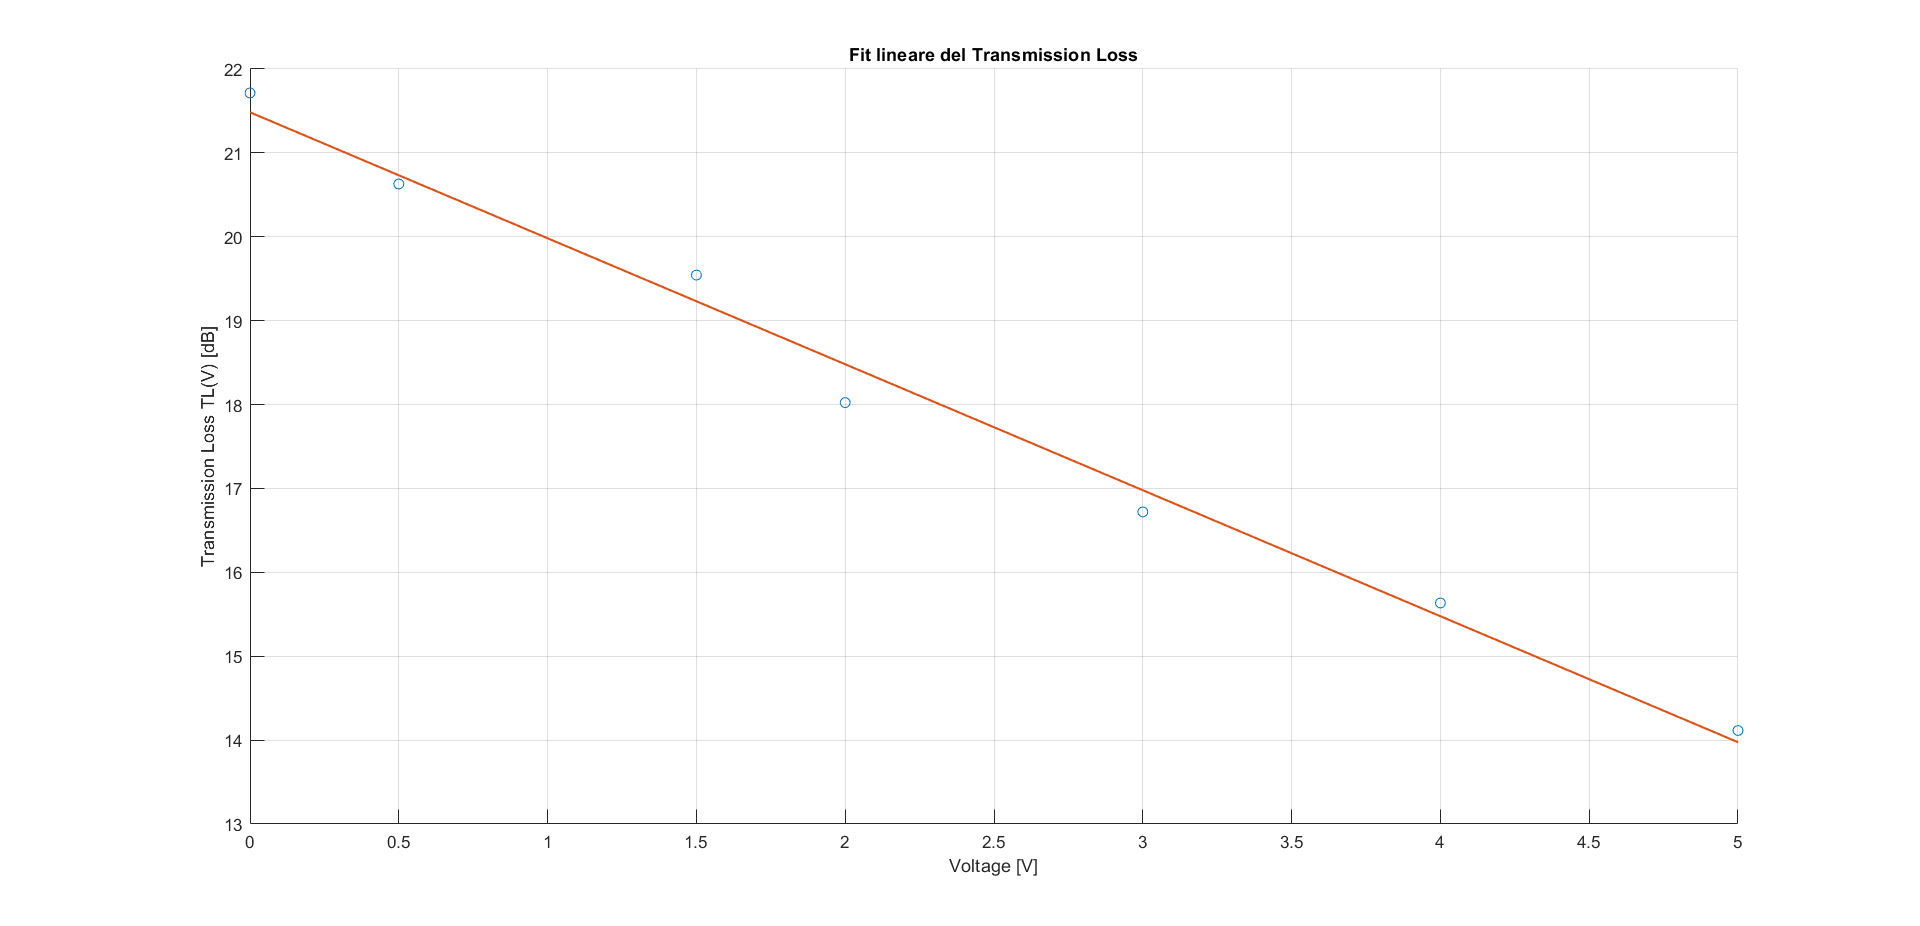
\includegraphics[width=\textwidth]{lab4/Images/fit_TL.png}
        \caption{Fit lineare di $TL_{dB}(V)$}
        \label{fig:fit_TL}
    \end{subfigure}
    \caption{Funzioni fittanti per $\Delta\phi(V)$ e $TL_{dB}(V)$ in funzione della tensione}
    \label{fig:fit_dphi_TL}
\end{figure}

\noindent\\ A partire dalle funzioni fittanti, è possibile calcolare i valori di $\Delta n_{eff}(V)$ e $\alpha_{tot}(V)$, definite dalle seguenti espressioni:
\begin{equation}\label{eq:d_neff}
\Delta n_{eff}(V) = \frac{\lambda}{2\pi} \cdot \frac{\Delta\phi(V)}{L}
\end{equation}
\noindent\\
\begin{equation}\label{eq:alfa_opt}
\alpha_{opt}(V) = \frac{TL_{dB}(V)}{L\cdot 10\log_{10}(e)}
\end{equation}

\noindent\\\\ Sfruttando le espressioni \ref{eq:d_neff} e \ref{eq:alfa_opt}, sono stati realizzati i grafici relativi alla variazione dell'indice di rifrazione efficace
$\Delta n_{eff}(V)$ e alla perdita $\alpha_{opt}(V)$ riportati nelle Figure \ref{fig:dneff_vs_V} e \ref{fig:alfa_opt_vs_V}.

\newpage

\begin{figure}[!h]
    \centering
    \begin{subfigure}[b]{0.49\textwidth}
        \centering
        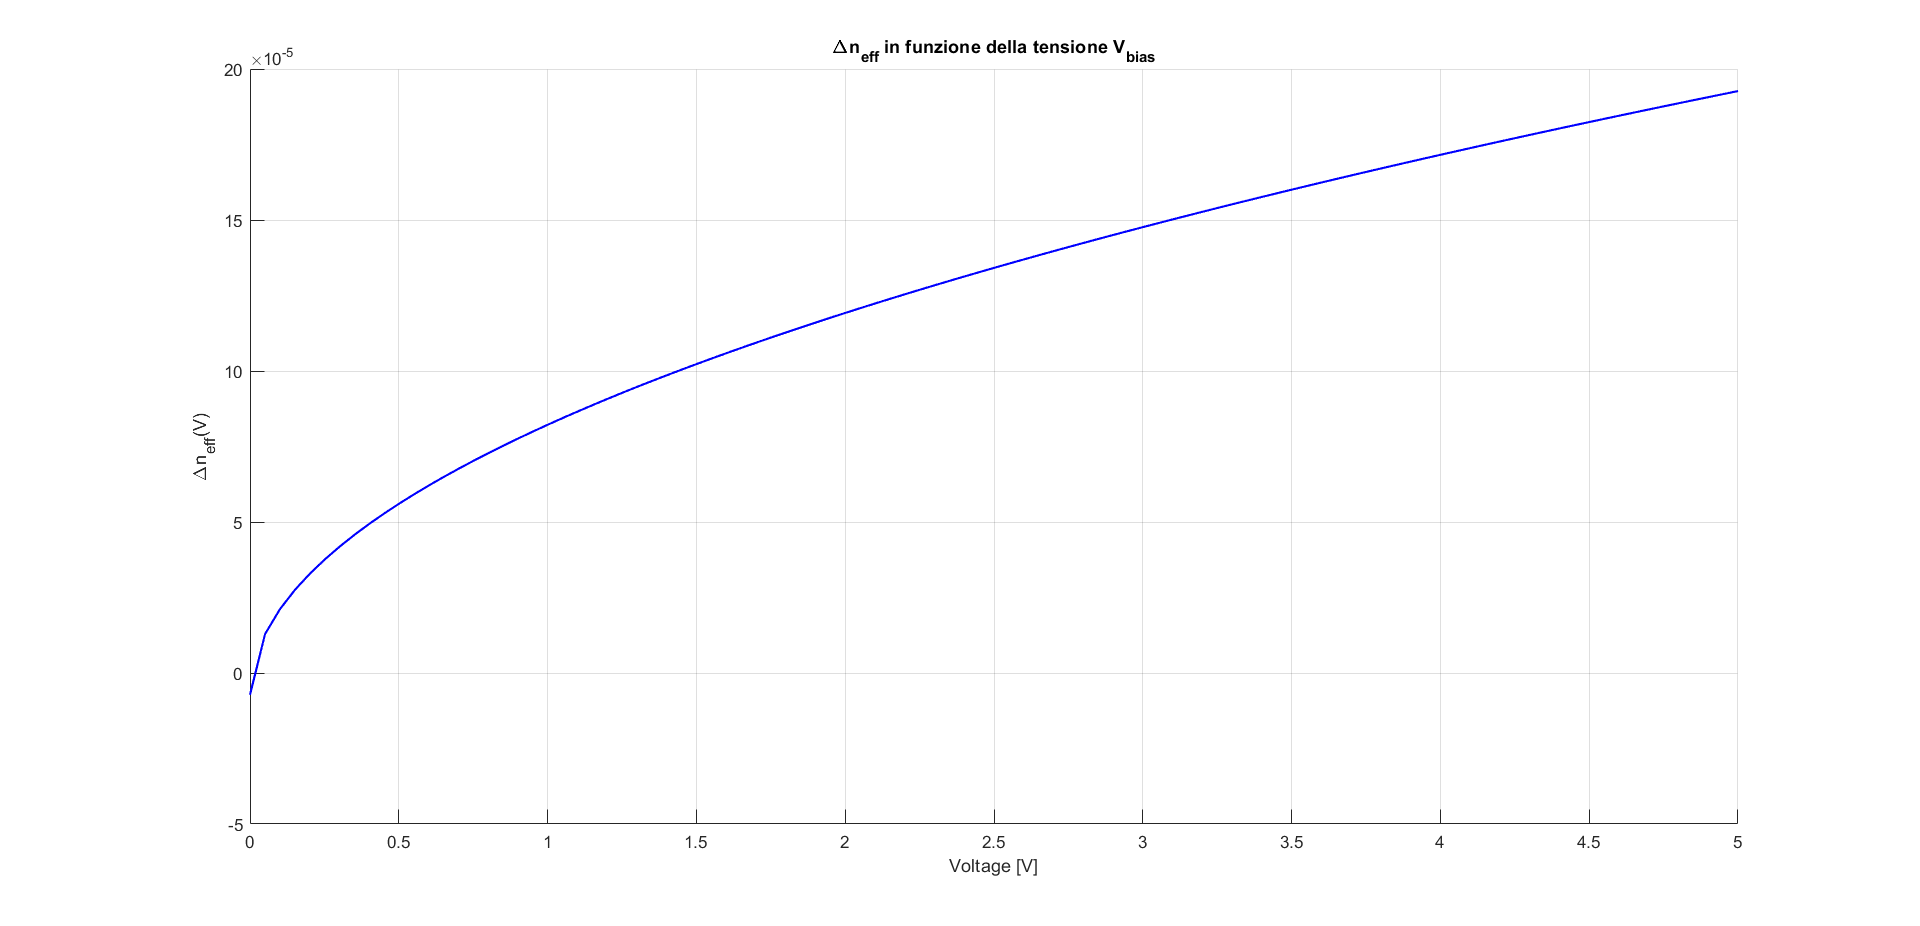
\includegraphics[width=\textwidth]{lab4/Images/dneff_vs_V.png}
        \caption{Variazione di $\Delta n_{eff}$ in funzione della tensione}
        \label{fig:dneff_vs_V}
    \end{subfigure}
    \hfill
    \begin{subfigure}[b]{0.49\textwidth}
        \centering
        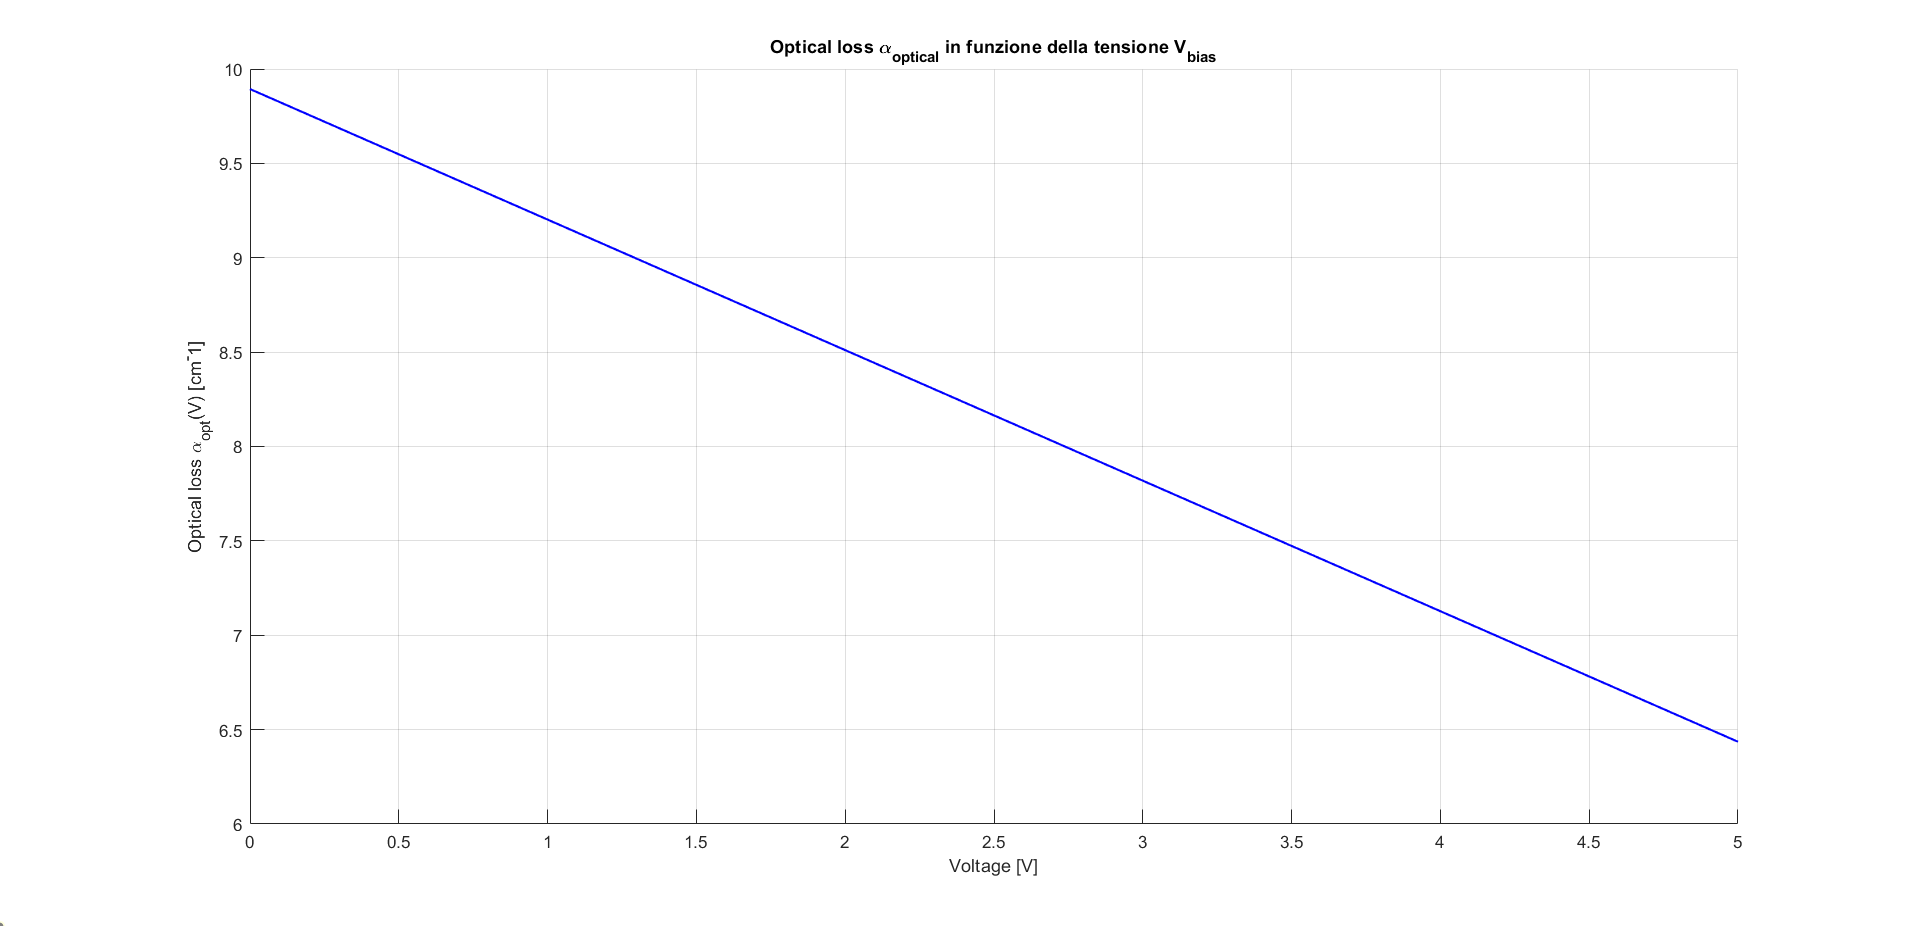
\includegraphics[width=\textwidth]{lab4/Images/alfa_opt_vs_V.png}
        \caption{Variazione di $\alpha_{opt}$ in funzione della tensione}
        \label{fig:alfa_opt_vs_V}
    \end{subfigure}
    \caption{Variazione di $\Delta n_{eff}$ e della perdita ottica $\alpha_{opt}$ in funzione della tensione}
    \label{fig:dneff_alfa_opt_vs_V}
\end{figure}

\noindent Dalla Figura \ref{fig:alfa_opt_vs_V} si può notare come l'optical loss diminuisca all'aumentare della tensione. Ciò accade a causa dell'allargamento
della zona di svuotamento che diminuisce la concentrazione di portatori liberi responsabili dell'assorbimento ottico attraverso il free-carrier effect.

\section{Calcolo dello spettro di trasmissione del modulatore}
\noindent Dopo aver stimato le perdite ottiche $\alpha_{opt}$ e la variazione di $n_{eff}$ con la tensione, si vuole calcolare lo spettro di trasmissione del modulatore,
definito come:
\begin{equation}\label{eq:transmission_spectrum}
    T(\lambda, V) = \frac{P_{out}(\lambda, V)}{P_{in}} = \left|\dfrac{E_1 + E_2}{\sqrt{2}}\right|^2
\end{equation}
\noindent L'intervallo di lunghezze d'onda d'interesse, in cui si vuole apprezzare la variazione di $T(\lambda, V)$, è compreso tra $1545 \text{ nm}$ e $1565 \text{ nm}$. Sono
state quindi valutate le espressioni dei due campi $E_1$ ed $E_2$, con il primo soggetto a una tensione $V$ variabile nell'intervallo tra $0 \text{ V}$ e $5 \text{ V}$, con passo
di $0.5 \text{ V}$. L'espressione del campo $E_1$ è la seguente:
\begin{equation}\label{eq:E1}
    E_1(\lambda, V) = \dfrac{\epsilon_{in}(t)}{\sqrt{2}} \cdot e^{-i \beta_1 L_1 - 0.5 \cdot \alpha_{tot,1} \cdot L_1}
\end{equation}
\noindent dove i termini dell'esponenziale $\beta_1$ e $\alpha_{tot,1}$ dipendono dalla tensione $V$ applicata.

\noindent\\ Per quanto riguarda il campo $E_2$, la sua espressione è la medesima; tuttavia, in questo caso, i termini dell'esponenziale $\beta_2$ e $\alpha_{tot,2}$ non
dipendono dalla tensione $V$, in quanto il ramo in questione non è polarizzato.

\noindent\\ L'andamento dello spettro di trasmissione $T(\lambda, V)$ in funzione della lunghezza d'onda e al variare della tensione applicata è riportato in
Figura \ref{fig:T_vs_lambda_V}.

\begin{figure}[!h]
 \centering
 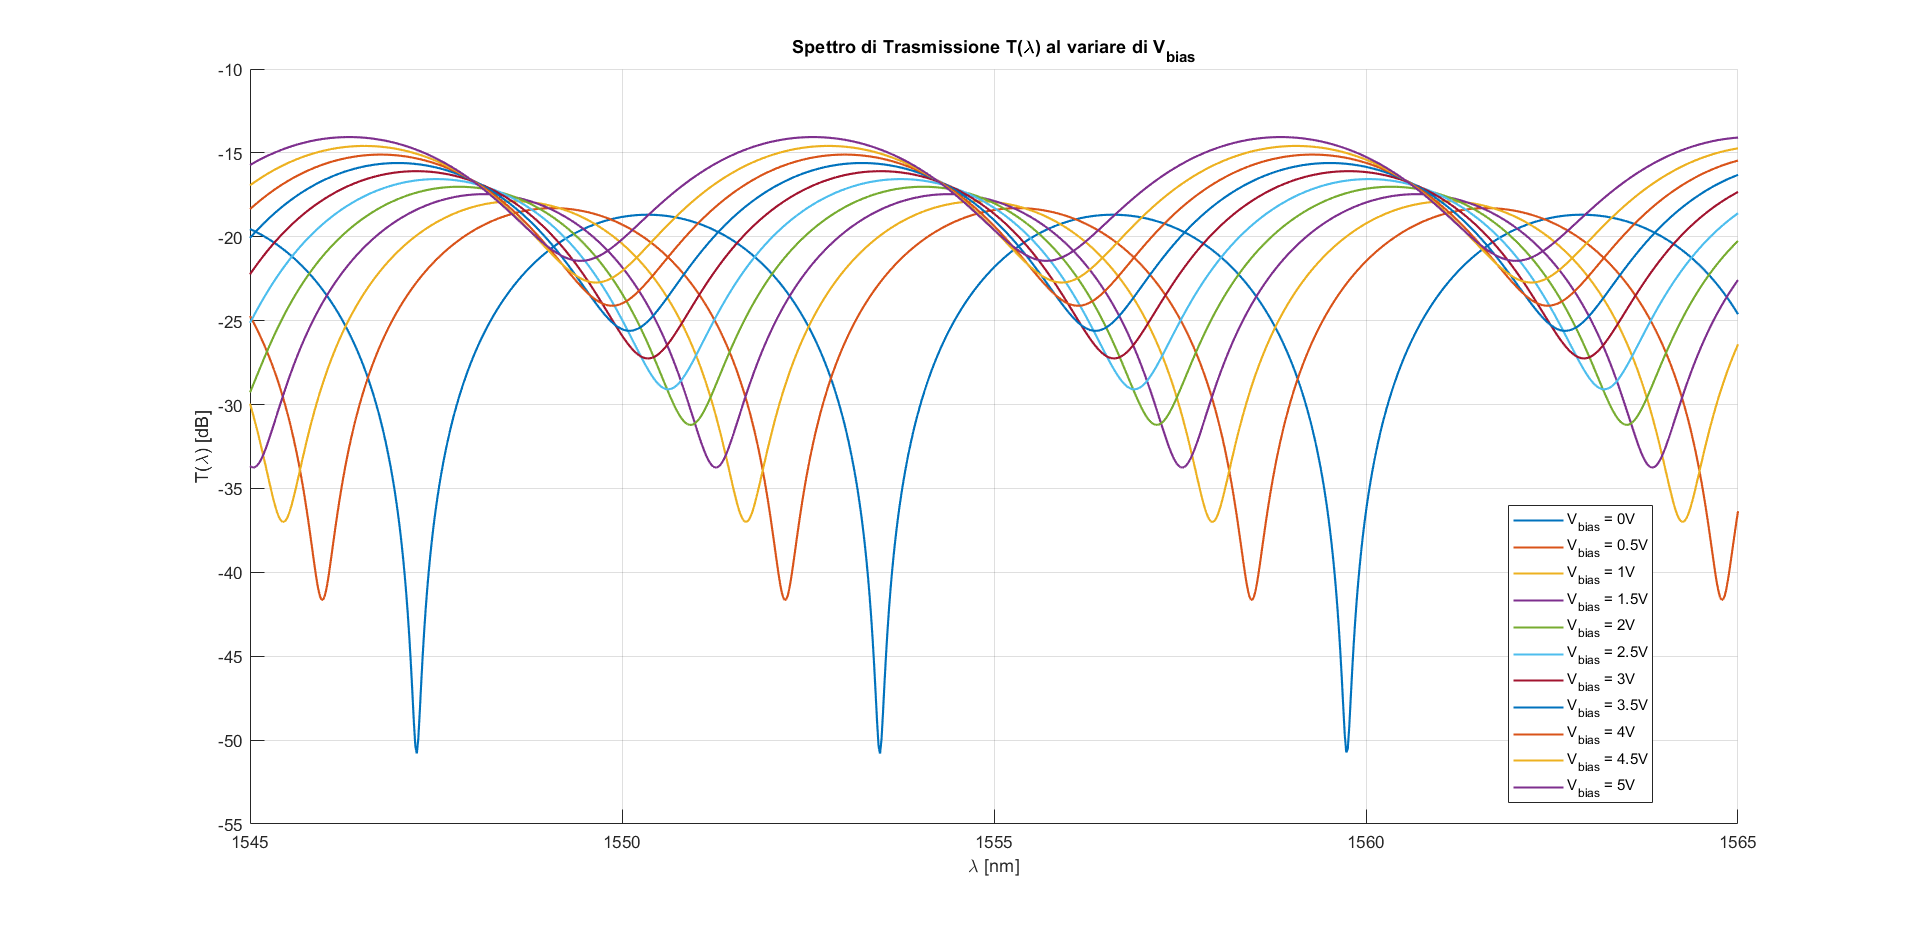
\includegraphics[width=15cm]{lab4/Images/T_vs_lambda_V.png}
  \caption{Spettro di trasmissione del modulatore MZI in funzione di $\lambda$ e $V$}
  \label{fig:T_vs_lambda_V}
\end{figure}

\noindent Come già accennato, la dipendenza dello spettro di trasmissione dalla lunghezza d'onda deriva dalla costante di propagazione.
\noindent In particolare, è possibile definire la costante di propagazione complessa $\tilde{\beta}$ per i due rami:
\begin{enumerate}
    \item Ramo polarizzato: $\tilde{\beta}_1 = \dfrac{2\pi}{\lambda} \left(n_{eff,0} + \Delta n_{eff}(V) \right) - i \dfrac{1}{2} \left(\alpha_{opt} + \Delta\alpha_{opt}(V)\right)$
    \item Ramo non polarizzato: $\tilde{\beta}_2 = \dfrac{2\pi}{\lambda} n_{eff,0} - i \dfrac{1}{2} \alpha_{opt}$
\end{enumerate}

\noindent Si evince che entrambi i rami presentino una dipendenza dalla lunghezza d'onda. Inoltre, dal grafico \ref{fig:T_vs_lambda_V} si può notare un aumento del modulo
dello spettro all'aumentare della tensione applicata; ciò è dovuto all'optical loss, che, come illustrato in precedenza, diminuisce all'aumentare la tensione.
Di conseguenza il campo che si propaga nel modulatore risulta attenuato dalle perdite della guida d'onda. Quindi, ipotizzando una guida d'onda ideale,
ossia senza perdite, si otterrebbe che il massimo della trasmissione raggiungerebbe idealmente $0 dB$, per qualsiasi valore di tensione applicata.

\section{Spettro di trasmissione in funzione della tensione di bias}
Dopo aver scelto una lunghezza d'onda $\lambda_{in} = 1550.34 \text{ nm}$, che corrisponde a un massimo di $T(\lambda, V = 0)$, si è
calcolato il coefficiente di trasmissione $T(\lambda, V = 0)$, facendo variare la tensione di bias da $0$ a $6 \,\text{V}$. L'andamento ottenuto è riportato in Figura \ref{fig:T_vs_Vbias} 

\begin{figure}[!h]
 \centering
 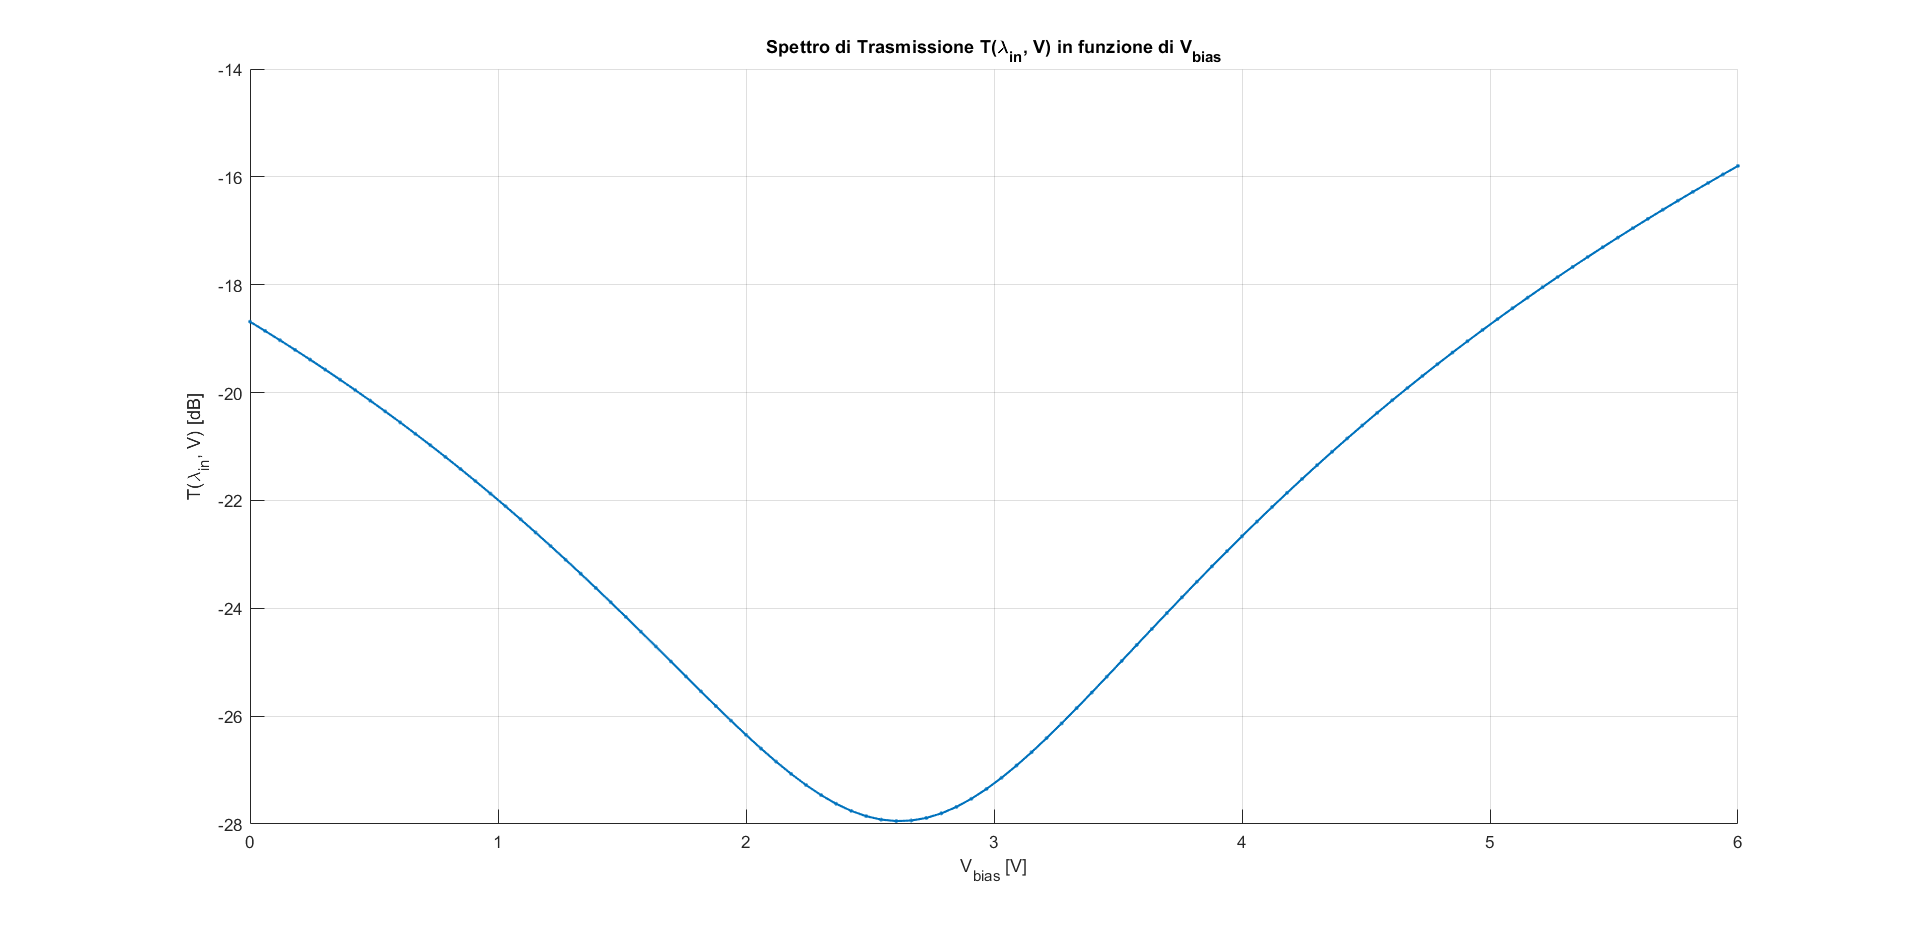
\includegraphics[width=15cm]{lab4/Images/T_vs_Vbias.png}
  \caption{Spettro di trasmissione con $\lambda_{in} = 1550.34 \text{ nm}$ fissa in funzione di $V$}
  \label{fig:T_vs_Vbias}
\end{figure}

\noindent Dalla figura sopra riportata è possibile ricavare il valore della tensione $V_{\pi}$, definita come la variazione di tensione necessaria per introdurre uno
sfasamento relativo di $\pi$ radianti tra i due rami del modulatore.

\noindent\\ Quando i campi ottici nei due rami si trovano in perfetta antifase, si verifica un'interferenza distruttiva che porta lo spettro di trasmissione al suo valore
minimo. Assumendo i due rami bilanciati a $0\text{ V}$, la tensione $V_{\pi}$ corrisponde alla tensione di polarizzazione in corrispondenza della quale si osserva il primo
minimo di trasmissione.

\noindent\\ Dal grafico in Figura \ref{fig:T_vs_Vbias} si evince che tale valore risulta pari a $V_{\pi} = 2{,}6061\text{ V}$.

\subsection{Calcolo dell'Extinction Ratio ER}
\noindent Noto il valore di $V_{\pi}$, è possibile calcolare l'Extinction Ratio (ER) del modulatore, definito come il rapporto tra la potenza ottica in uscita quando si trasmette
il livello alto (bit $"1"$) e la potenza ottica in uscita quando si trasmette il livello basso (bit $"0"$). Questo valore è un indicatore della qualità del modulatore: 
un ER maggiore indica una migliore separazione tra i due livelli.
\noindent\\ Assumendo di avere una tensione modulante con ampiezza picco-picco pari a $V_{pp}$, si può definire l'Extinction Ratio tramite la seguente espressione:

\begin{equation}\label{eq:ER}
    ER = \dfrac{P_{"1"}}{P_{"0"}} = \dfrac{T(V_{bias} - V_{pp}/2)}{T(V_{bias} + V_{pp}/2)}, \text{ nel caso di } V_{bias} < V_{\pi}
\end{equation}
\noindent\\
\begin{equation}\label{eq:ER2}
    ER = \dfrac{P_{"1"}}{P_{"0"}} = \dfrac{T(V_{bias} + V_{pp}/2)}{T(V_{bias} - V_{pp}/2)}, \text{ nel caso di } V_{bias} > V_{\pi}
\end{equation}

\noindent\\ L'andamento dell'Extinction Ratio ER in funzione della tensione di bias è riportato in Figura \ref{fig:ER_vs_Vbias}.

\begin{figure}[!h]
 \centering
 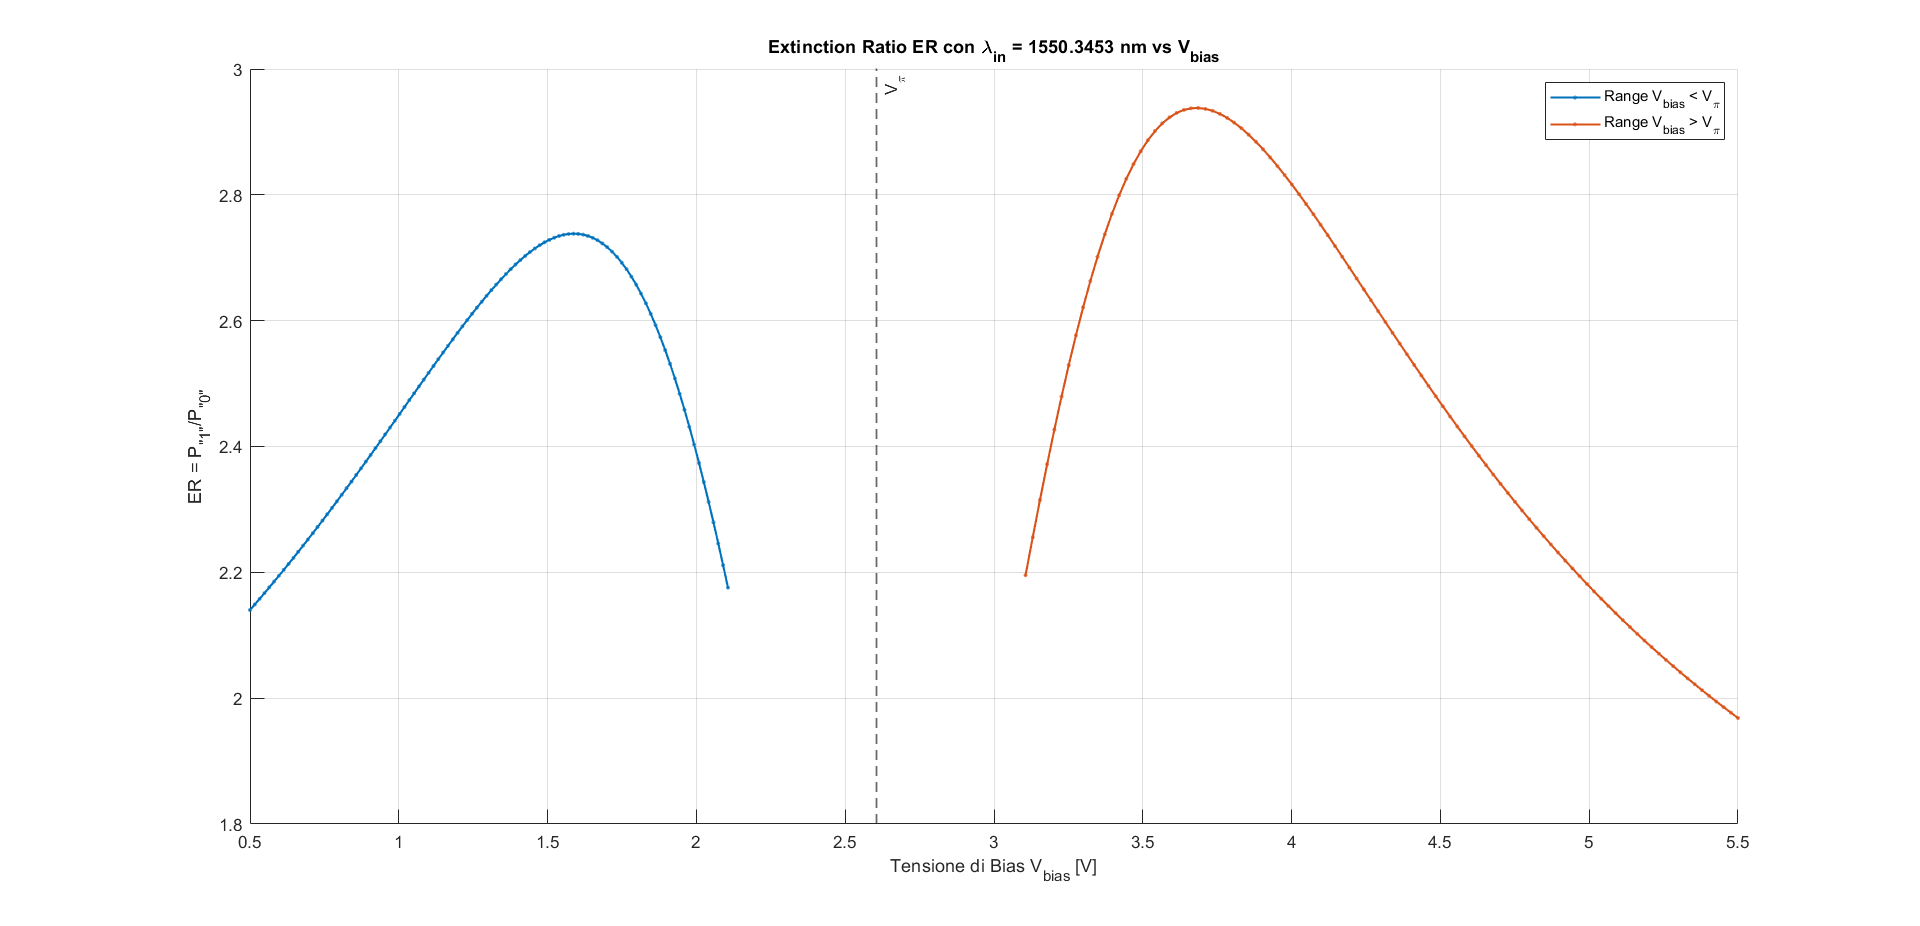
\includegraphics[width=12.5cm]{lab4/Images/ER_vs_Vbias.png}
  \caption{Extinction Ratio in funzione della tensione di bias $V$}
  \label{fig:ER_vs_Vbias}
\end{figure}

\noindent Dal grafico sopra riportato, si evince che il picco massimo dell'Extinction Ratio si ottiene per una tensione di bias pari a $V_{bias} = 3.6864\text{ V}$, che risulta
essere il valore ottimale per il funzionamento del modulatore. Tale valore è quindi superiore al valore di $V_{\pi}$; questa caratteristica era già intuibile dal grafico
del coefficiente di trasmissione $T(\lambda_{in}, V)$ in Figura \ref{fig:T_vs_Vbias}, in quanto il tratto della caratteristica a destra di $V_{\pi}$ presenta una pendenza
più ripida e, di conseguenza, una maggiore differenza tra le due potenze in uscita (stato ON e OFF).

\noindent\\ Come ultima analisi si è calcolata la perdita al livello $"1"$ in funzione della tensione di bias.

\begin{figure}[!h]
 \centering
 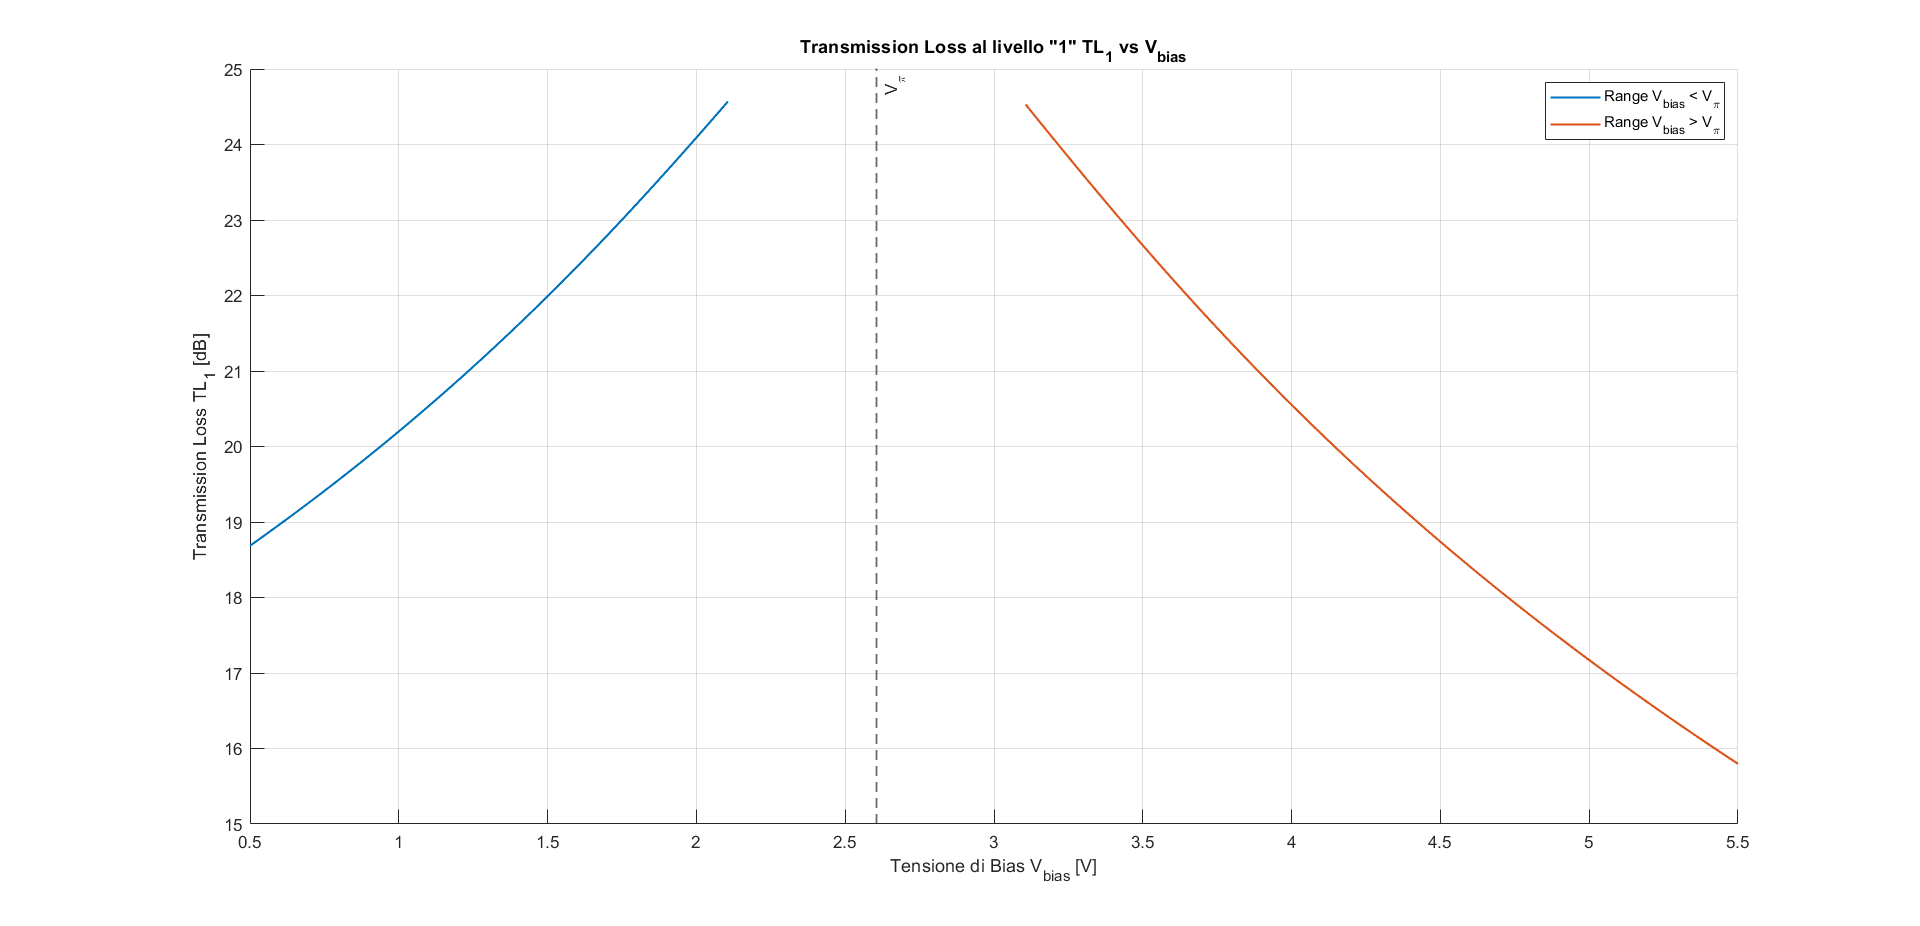
\includegraphics[width=12.5cm]{lab4/Images/TL1_vs_Vbias.png}
  \caption{Perdita di trasmissione al livello "1" in funzione della tensione di bias $V$}
  \label{fig:TL1_vs_Vbias}
\end{figure}

\noindent Dalla Figura \ref{fig:TL1_vs_Vbias} si osserva che la perdita di trasmissione $TL_1$ aumenta progressivamente man mano che la tensione di bias si avvicina al valore $V_{\pi}$,
dove si registra il massimo dell'attenuazione. Questo comportamento è legato alla risposta dell'interferometro: impostando $V_{\text{bias}}$ prossimo a $V_{\pi}$, il punto
di lavoro del modulatore si sposta in prossimità del minimo della curva di trasmissione (dove avviene l'interferenza distruttiva), riducendo di conseguenza la potenza ottica
associata al livello logico "1". Allontanandosi da $V_{\pi}$, il punto di lavoro si riallinea verso zone a maggiore trasmissione ottica, determinando una netta
riduzione delle perdite.

\section{Larghezza di banda del modulatore}
L'obiettivo di quest'analisi è osservare l'impatto delle perdite della linea di trasmissione, del disadattamento di velocità di fase e della resistenza di terminazione
sulla larghezza di banda di modulazione di questo modulatore. Dalle formule riportate nella consegna sono state ricavate le espressioni per calcolare la risposta in
frequenza del modulatore $\boldsymbol{m(f)}$ nel caso generale con $Z_g$ non nullo, impedenza di carico $Z_L$, disadattamento della velocità di fase e perdite non nulle
della microstrip coplanare. La risposta in frequenza del modulatore
\begin{equation}
    m(f) = \dfrac{|\Delta\phi(f)|}{\Delta\phi(0)} 
\end{equation}
rappresenta quanto la fase è modulata ad una certa frequenza rispetto alla modulazione massima che si ha per $f=0$.

\noindent\\ In una prima analisi, si è messo in evidenza il ruolo del \textbf{disadattamento della velocità di fase} tra il campo ottico e il segnale a micro-onde,
considerando quindi trascurabili le perdite della microstrip.

\noindent\\ L'andamento ottenuto è riportato in Figura \ref{fig:m_vs_f_dv}

\begin{figure}[!h]
 \centering
 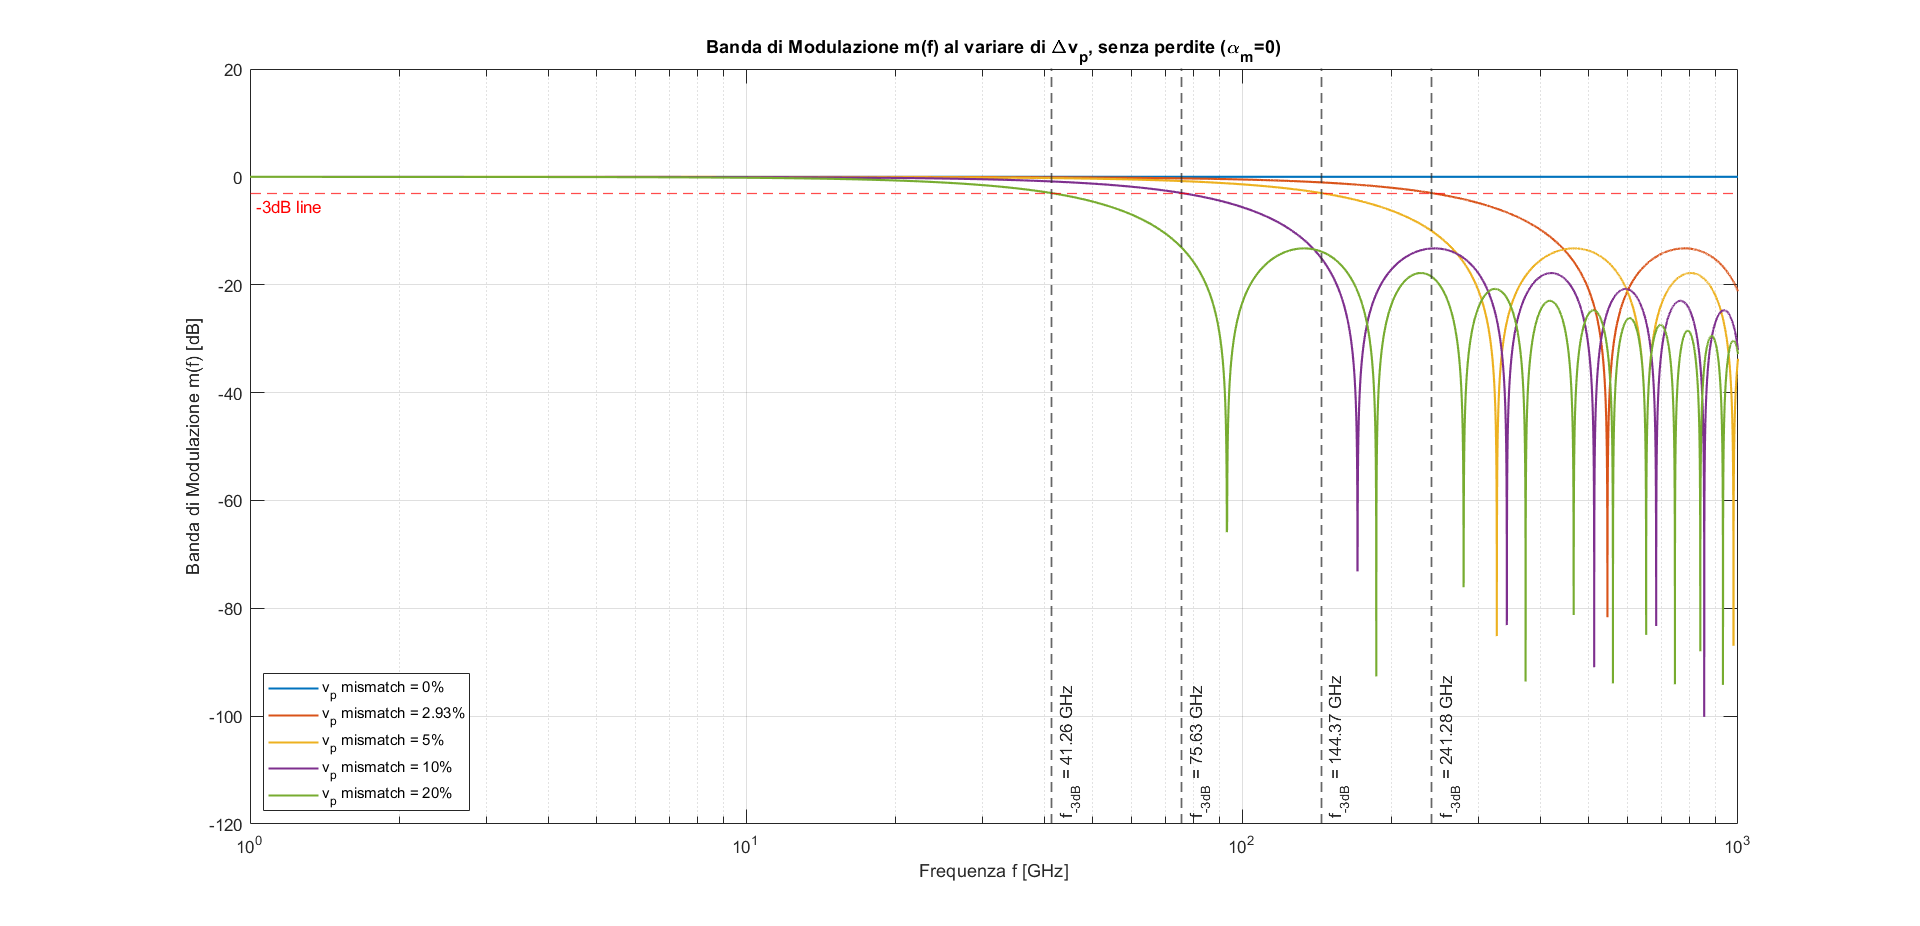
\includegraphics[width=15cm]{lab4/Images/m_vs_f_dv.png}
  \caption{Risposta in frequenza del modulatore al variare del velocity mismatch con $\alpha_m=0$}
  \label{fig:m_vs_f_dv}
\end{figure}

\noindent Dalla Figura \ref{fig:m_vs_f_dv} si evince che la banda a $-3 \,\text{dB}$ del modulatore diminuisca all'aumentare del disadattamento della velocità di fase,
in particolare passa da circa $f_{-3\,\text{dB}} \approx 240 \text{ GHz}$ con il velocity mismatch nominale ($\Delta v \approx 2.93\%$) a circa $f_{-3\,\text{dB}} \approx 40 \text{ GHz}$
con un mismatch ($\Delta v \approx 20\%$). Inoltre, si noti come, con un mismatch nullo ($\Delta v = 0$), la banda del modulatore risulti idealmente infinita, in quanto 
in questa analisi non è stato incluso alcun termine di perdita.

\newpage
\noindent In una seconda analisi, si è messo in evidenza il ruolo delle \textbf{perdite della microstrip}, considerando anche il disadattamento nominale della velocità di fase.
La risposta in frequenza ottenuta è riportata in Figura \ref{fig:m_vs_f_am}

\begin{figure}[!h]
 \centering
 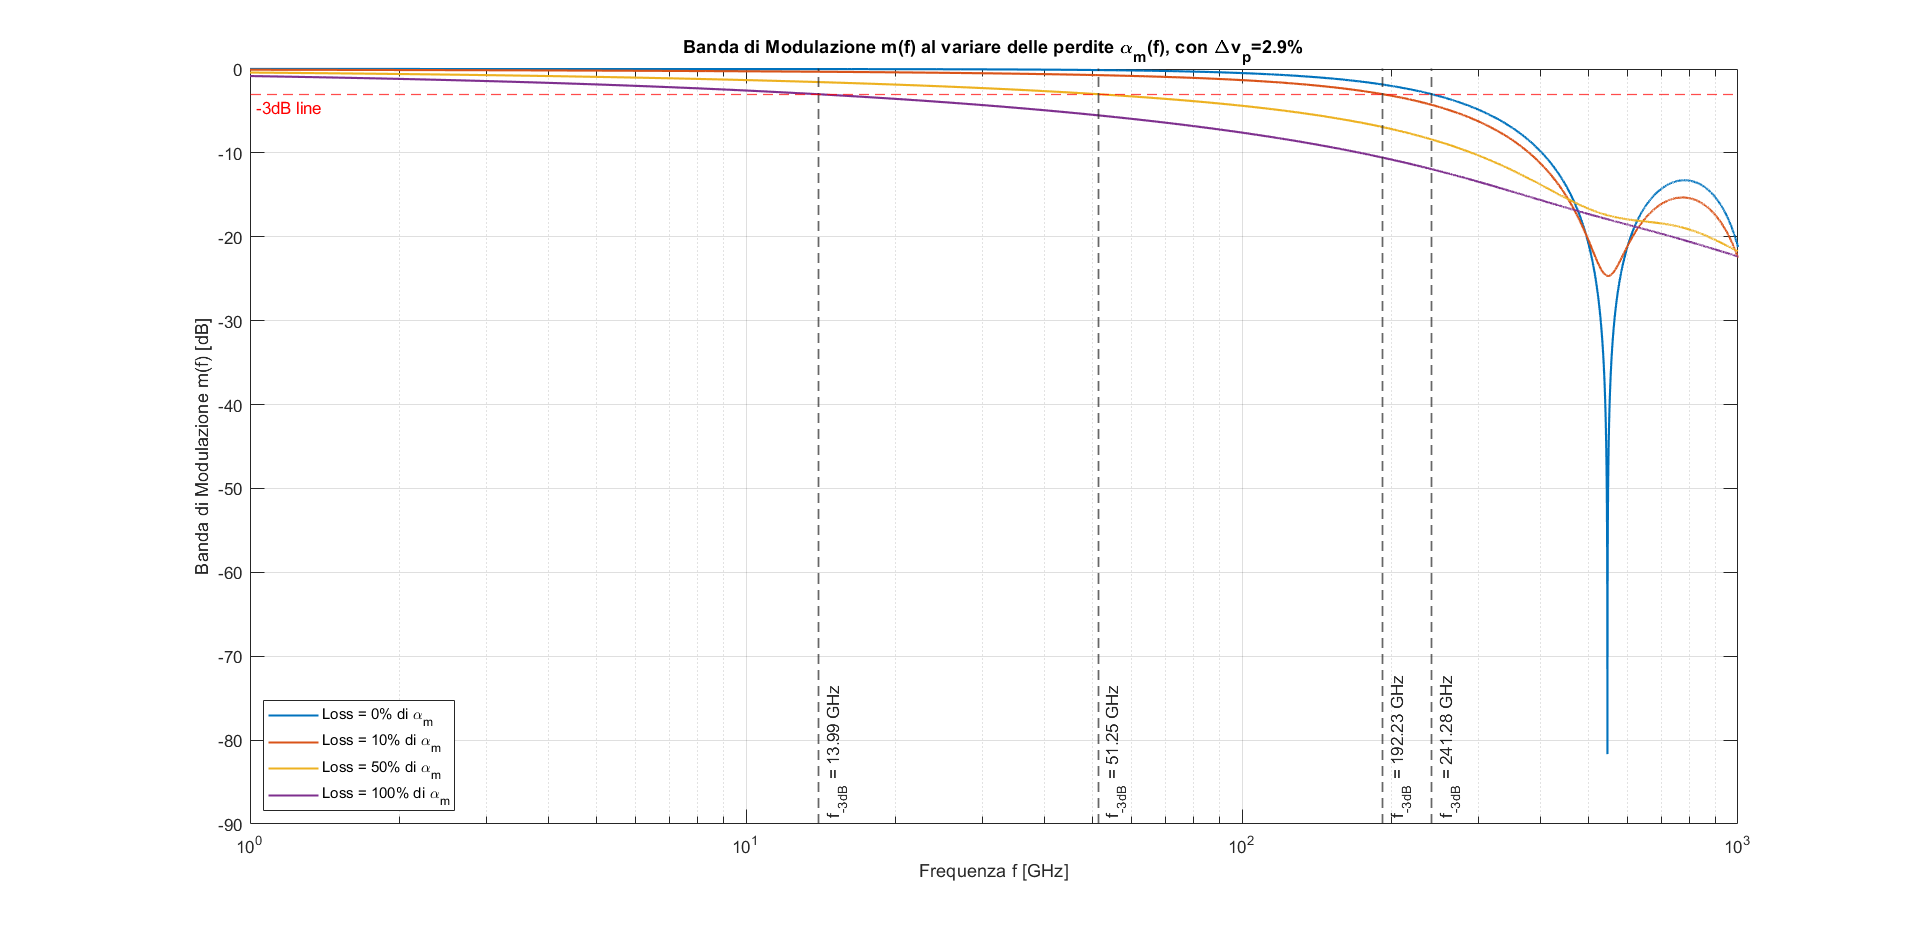
\includegraphics[width=12.5cm]{lab4/Images/m_vs_f_am.png}
  \caption{Risposta in frequenza del modulatore al variare delle perdite con $\Delta v = 2.93\%$}
  \label{fig:m_vs_f_am}
\end{figure}

\noindent Per valutare al meglio l'impatto delle perdite della microstrip, si è introdotto un fattore moltiplicativo (che varia da $0$ a $1$) che moltiplica il valore nominale
delle perdite della microstrip.

\noindent\\ Dalla Figura \ref{fig:m_vs_f_am} si evince che la banda a $-3 \,\text{dB}$ del modulatore diminuisca vertiginosamente all'aumentare delle
perdite della microstrip, in particolare passa da circa $f_{-3\,\text{dB}} \approx 240 \text{ GHz}$ con il fattore moltiplicativo pari a 0 (quindi, caso senza perdite, ma 
con solo velocity mismatch $\Delta v = 2.93\%$) a circa $f_{-3\,\text{dB}} \approx 50 \text{ GHz}$ con un fattore moltiplicativo pari a $0.5$.

\noindent\\ Includendo le perdite nominali della microstrip (coefficiente moltiplicativo pari a $1$), la banda a $-3 \,\text{dB}$ del modulatore risulta essere 
$f_{-3\,\text{dB}} \approx 14 \text{ GHz}$, quindi circa il $6\%$ della banda originale.

\subsubsection{Calcolo dell'energia per bit}
Infine si è calcolato il costo di energia per bit, assumendo che il modulatore sia modulato con un bit-rate uguale alla massima banda a $-3 \,\text{dB}$ nel grafico precedente
e che la tensione picco-picco $V_{pp} = 1 \text{V}$. Ne consegue che $BW_{max} = 241 \text{ GHz}$ e $V_{pk} = V_{pp}/2 = 0.5 \text{V}$.

\noindent\\ La potenza richiesta per pilotare il modulatore è pari a:
\begin{equation}
    P_{RF} = \dfrac{V_{pk}^2}{2 Z_g} \cdot \dfrac{1}{1 - \Gamma_g^2}
\end{equation}
\noindent dove:
\begin{equation}
    \Gamma_g = \dfrac{Z_g - Z_0}{Z_g + Z_0}
\end{equation}

\noindent\\ Svolgendo i calcoli, si trova che il costo energetico per bit è pari a:
\begin{equation}
    E_{bit} = \dfrac{P_{RF}}{BW_{max}} = 10.598 \text{ fJ/bit}
\end{equation} 
